\chapter{Fussballszenario} \label{kap:Fussballszenario} %TODO: Besseren Kapiteltitel

\section{Szenario Koordination} %TODO: Hendrik

\subsection{Kommunikation per RSB und Spread} %TODO: Hendrik

\subsection{Finite-State-Machine} %TODO: Hendrik

\begin{figure}[H]
	\begin{center}
		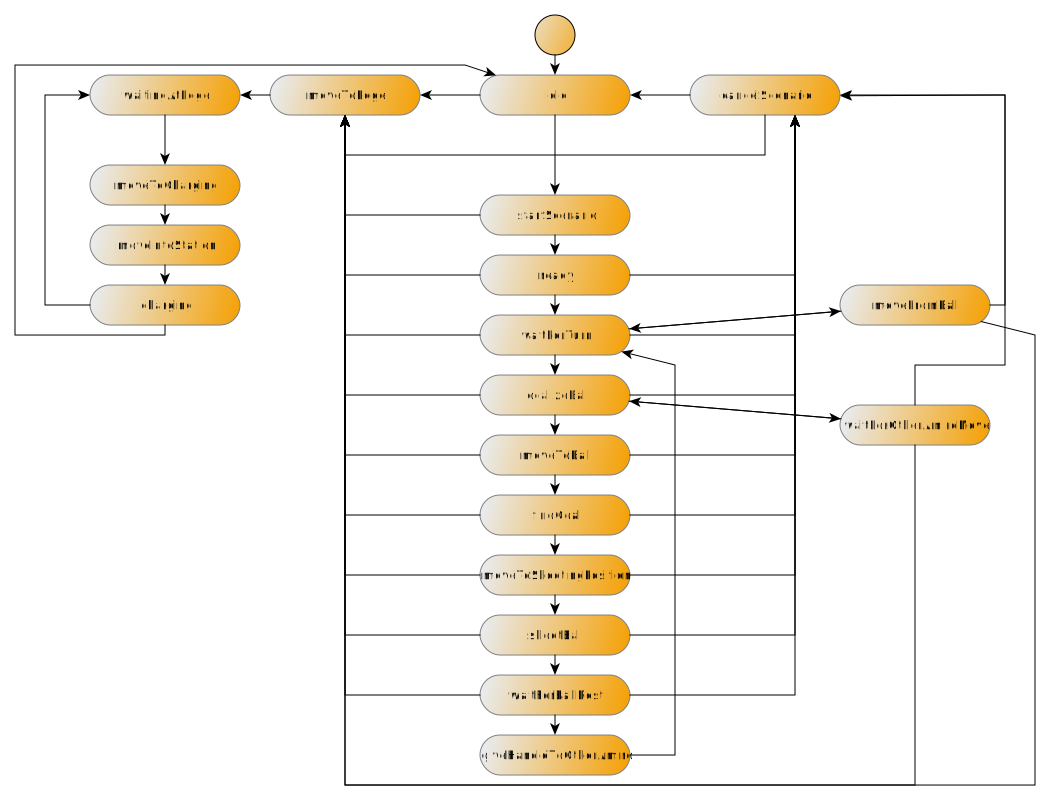
\includegraphics[scale=.55]{Final_FSM_AMiRo.pdf} 	
		\caption{Finite-State-Machine}
		\label{fig:fsm-amiro}
	\end{center}
\end{figure}

\section{Realisierung der einzelnen Spielelemente} %TODO: Besseren Sectiontitel

\subsection{Lokalisation des Balls} %TODO: Julian E.

\subsection{Anfahren des Balls} %TODO: Julian E.

\subsection{Lokalisation des gegnerischen Tores} %TODO: Timo M.
- Rotation um eigene Achse zur Lokalisation des Tores
- Lokalisation Anhand von Blobb-Detektion 
- Wenn ein einzelner Pfosten im Bild vorhanden ist - bereits gedrehten Winkel + zusätlichen Winkel vom Mittelpunkt des Bildes zum Pfosten speichern
- Wenn beide Pfosten im Bild vorhanden sind - bereits gedrehten Winkel + zusätlichen Winkel vom Mittelpunkt des Bildes zum Tormittelpunkt speichern und Rotation beenden
- Drehung zum Ball durchführen, um diesen wieder vor sich zu haben

\subsection{Schussposition anfahren} %TODO: Timo M.
- Je nach Winkel zum Tor entscheiden, ob der Ball links- oder rechtsseitig umfahren werden soll
- 90$^\circ$ Drehung zu der gegebenen Seite 
- Umfahren des Balles bis vorher berechneter Winkel zum Tor erreicht ist
	- Bei einem Hindernis wird das Umfahren des Balles gestoppt
- 90$^\circ$ Drehung zum Ball
- Überprüfung, ob sowohl Ball als auch das Tor im Bild zu sehen ist 
	- Ist dies der Fall -> feinjustierung der Schussposition 

\subsection{Schießen} %TODO: Timo M.
- Überprüfen der seitlichen vorderen Abstandssensoren ob eine Wand detektiert wird
	- Sollte eine Wand auf einer Seite detektiert werden -> Angedrehter Schuss mit Drehung des AMiRos weg von der Wand
- Schießen des Balles durch kurzes Ansteuern beider Motoren 

\subsection{Beiseite Fahren} %TODO: Julian E. (Besseren Titel suchen^^)

\section{Spieltracking} %TODO: Julian D.

\subsection{Spielfeldbestimmung mit dem AR Toolkit} %TODO: Julian D.

\subsection{Extraktion wichtiger Spielelemente mit Bildverarbeitungsmethoden} %TODO: Julian D.

\subsection{Benutzerinteraktion mit AR Markern} %TODO: Julian D.

\subsection{Spielkoordination} %TODO: Julian D.

\subsection{Grafische Darstellung der Spielstatus} %TODO: Julian D.